\documentclass[12pt]{article}
\usepackage[utf8]{inputenc}

\usepackage{color,soul}
\usepackage{xcolor}
\usepackage{array}
\usepackage{mhchem}
\usepackage{mathtools}

\DeclarePairedDelimiter\ceil{\lceil}{\rceil}
\DeclarePairedDelimiter\floor{\lfloor}{\rfloor}

\bibliographystyle{plos2015}


\begin{document}


\section*{S2 Appendix: Well-calibrated simulation studies}


Every method presented and tested in this paper was validated with a well-calibrated simulation study using the same model and operator set that which was benchmarked. This is achieved using 100 simulated datasets (each with $N=100$ taxa and a $L=5000$ nt alignment). The 95 \% highest posterior density (HPD) interval is calculated, and the `true' parameter values are compared with their values estimated from the simulated data. 


The validation results are presented as plots. The number in the bottom right corner of each plot is the coverage; that is the percentage of simulations where the `true' parameter value is within the 95 \% HPD interval. If all parameters have coverage close to 95 \% coverage, then this suggests correctness of implementation.


The parameters presented in each plot are: the Yule model birth rate $\lambda$, rate heterogeneity gamma shape $\Gamma$, HKY substitution model parameter $\kappa$, log-normal clock standard deviation $\sigma$, the frequency of the A nucleotide $f_A$, and the rate of the first taxon $r_1$. The remaining 3 frequencies and 99 taxa rates are omitted from the figures. 




\begin{figure}[!htb]
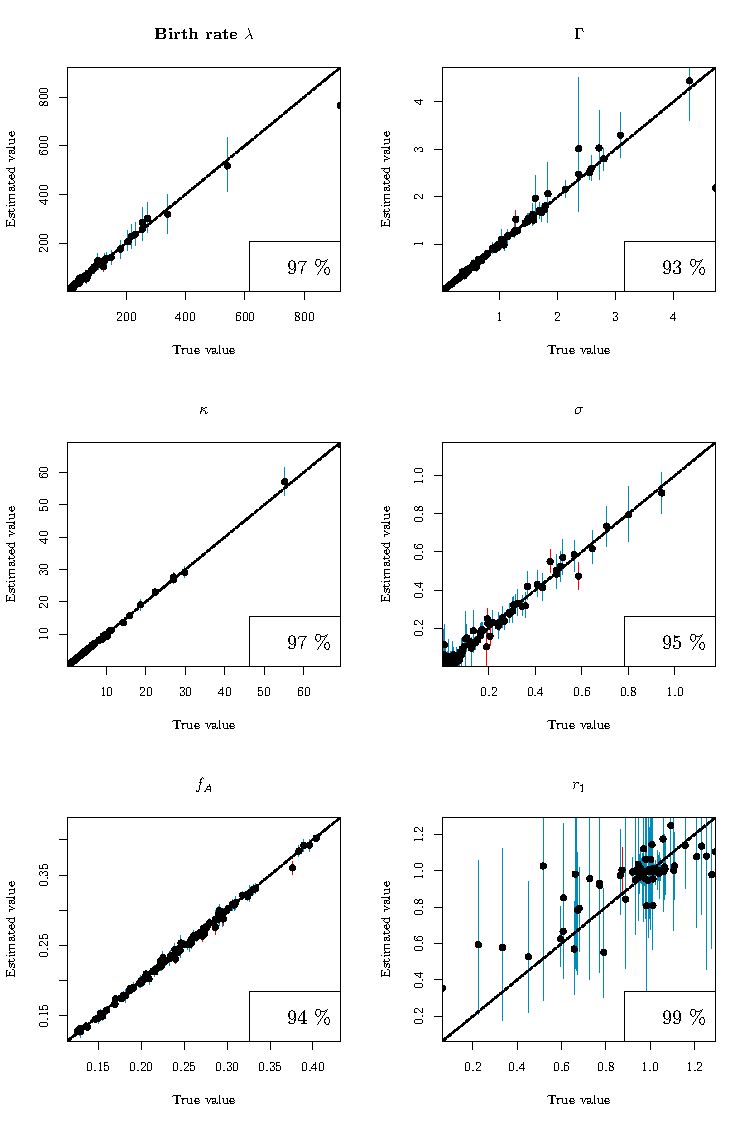
\includegraphics[width=0.85\textwidth]{Figures/CalSim_cat.pdf}
\caption{\textbf{The \textit{cat} parameterisation.} Blue and red vertical lines are 95 \% HPD intervals, where blue intervals contain the true value and red intervals do not.}
\label{fig:rateparams}
\end{figure}


\begin{figure}[!htb]
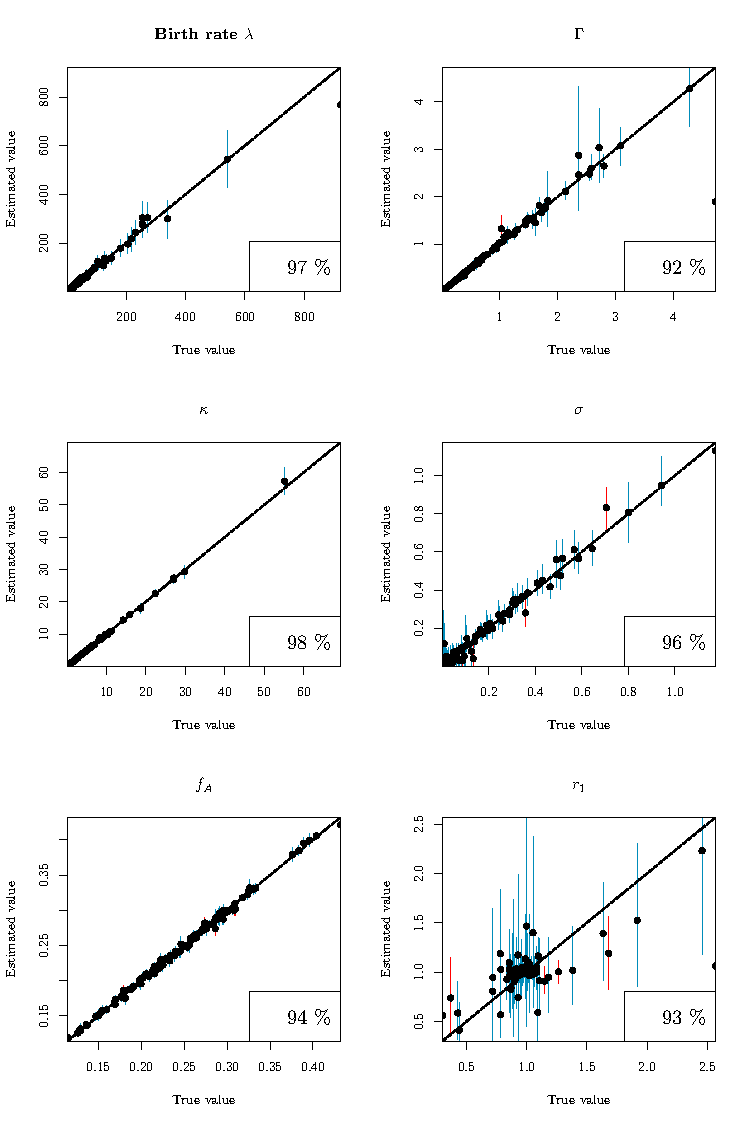
\includegraphics[width=0.85\textwidth]{Figures/CalSim_real.pdf}
\caption{\textbf{The \textit{real} parameterisation,} with the operators decribed by Zhang and Drummond 2020. The \textit{real 2006} setting uses a subset of the operators tested in this validation. }
\label{fig:rateparams}
\end{figure}


\begin{figure}[!htb]
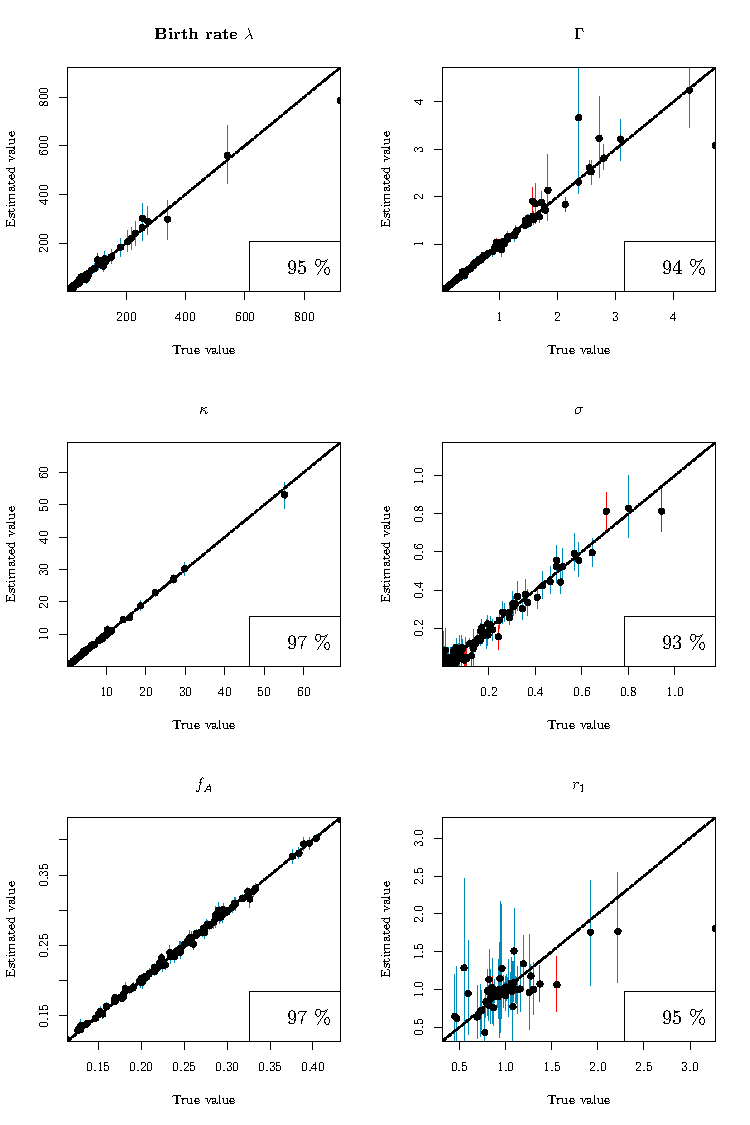
\includegraphics[width=0.85\textwidth]{Figures/CalSim_quant.pdf}
\caption{\textbf{The \textit{quant} parameterisation,} with the operators decribed by Zhang and Drummond 2020, and adapted for \textit{quant} as described in \textbf{S1 Appendix}. The \textit{quant 2006} setting uses a subset of the operators tested in this validation.}
\label{fig:rateparams}
\end{figure}



\begin{figure}[!htb]
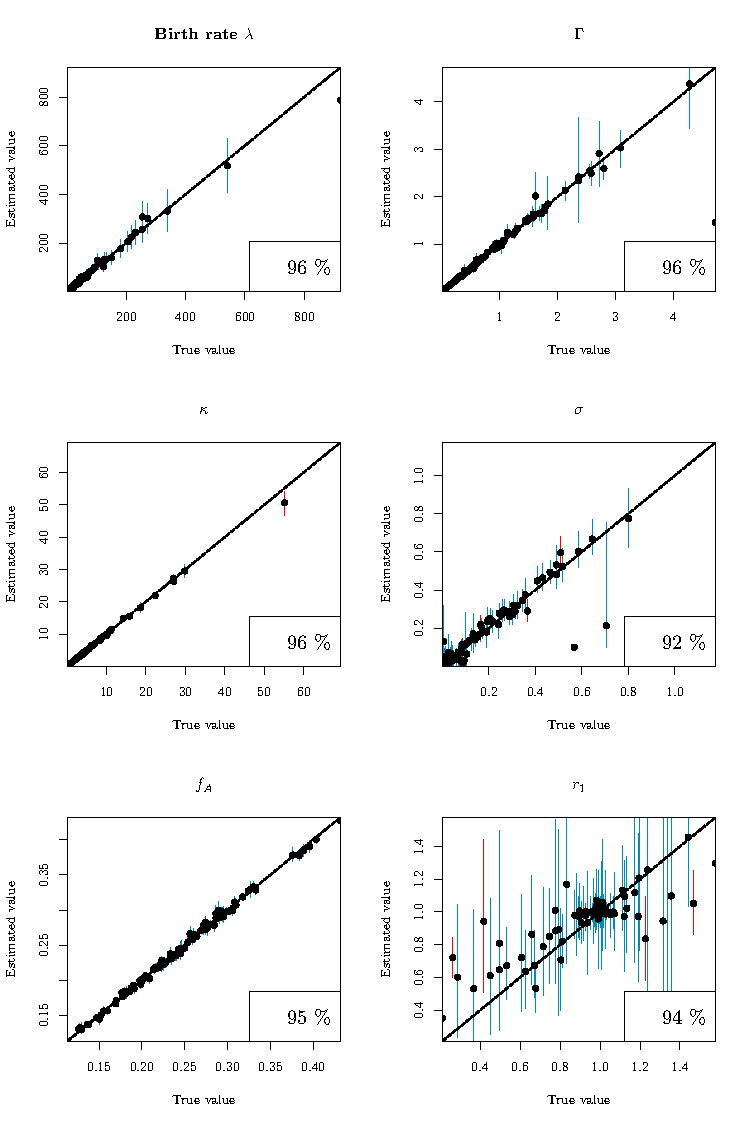
\includegraphics[width=0.85\textwidth]{Figures/CalSim_NER_real.pdf}
\caption{\textbf{The Narrow Exchange Rate operators under the \textit{real} parameterisation.} The 48 NER and 48 NERw operators, including the null Narrow Exchange operator, are tested in the same MCMC session.}
\label{fig:rateparams}
\end{figure}



\begin{figure}[!htb]
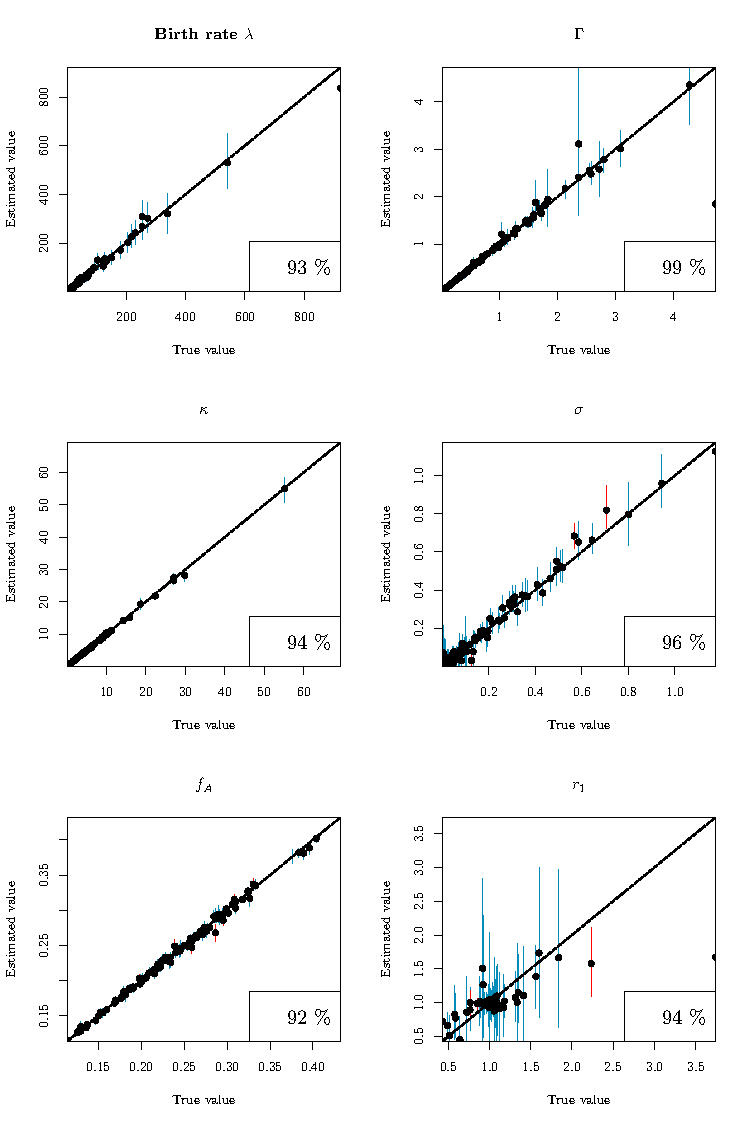
\includegraphics[width=0.85\textwidth]{Figures/CalSim_NER_quant.pdf}
\caption{\textbf{The Narrow Exchange Rate operators under the \textit{quant} parameterisation.} The 48 NER and 48 NERw operators are tested simultaneously.}
\label{fig:rateparams}
\end{figure}




\begin{figure}[!htb]
%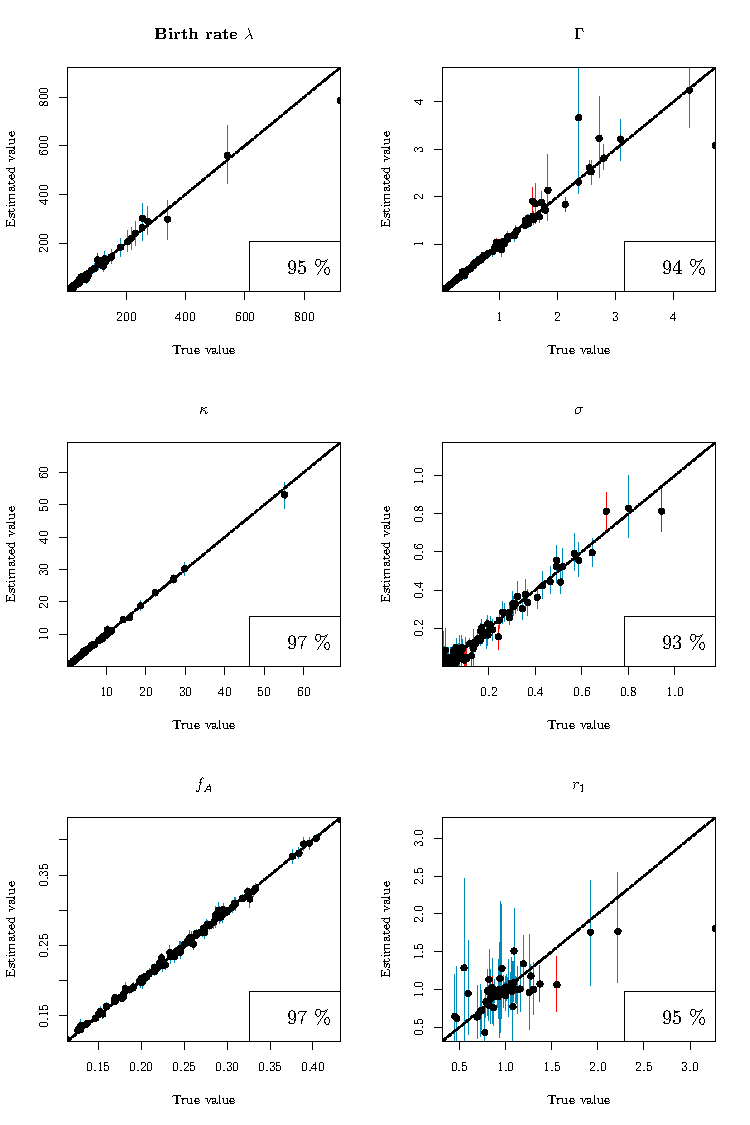
\includegraphics[width=0.85\textwidth]{Figures/CalSim_quant.pdf}
\caption{\textbf{Bactrian proposal kernel.} A $\text{Bactrian}(0.95)$ proposal kernel is used for all clock model operators, as described in main article.}
\end{figure}





\bibliography{references}




\end{document}